% !Mode:: "TeX:UTF-8"
%!TEX program = xelatex

\documentclass[withoutpreface,bwprint]{cumcmthesis}

\usepackage{float}
\usepackage{subfigure}
\usepackage{multirow}
\usepackage{longtable}
\usepackage{enumerate}
\usepackage{diagbox}
\usepackage{float}
\title{颜色与物质浓度辨识}
\tihao{C}
\membera{严宋扬}
\membera{汪紫薇}
\membera{袁靖松}


\begin{document}
 %%封面
\begin{titlepage}
\centering
%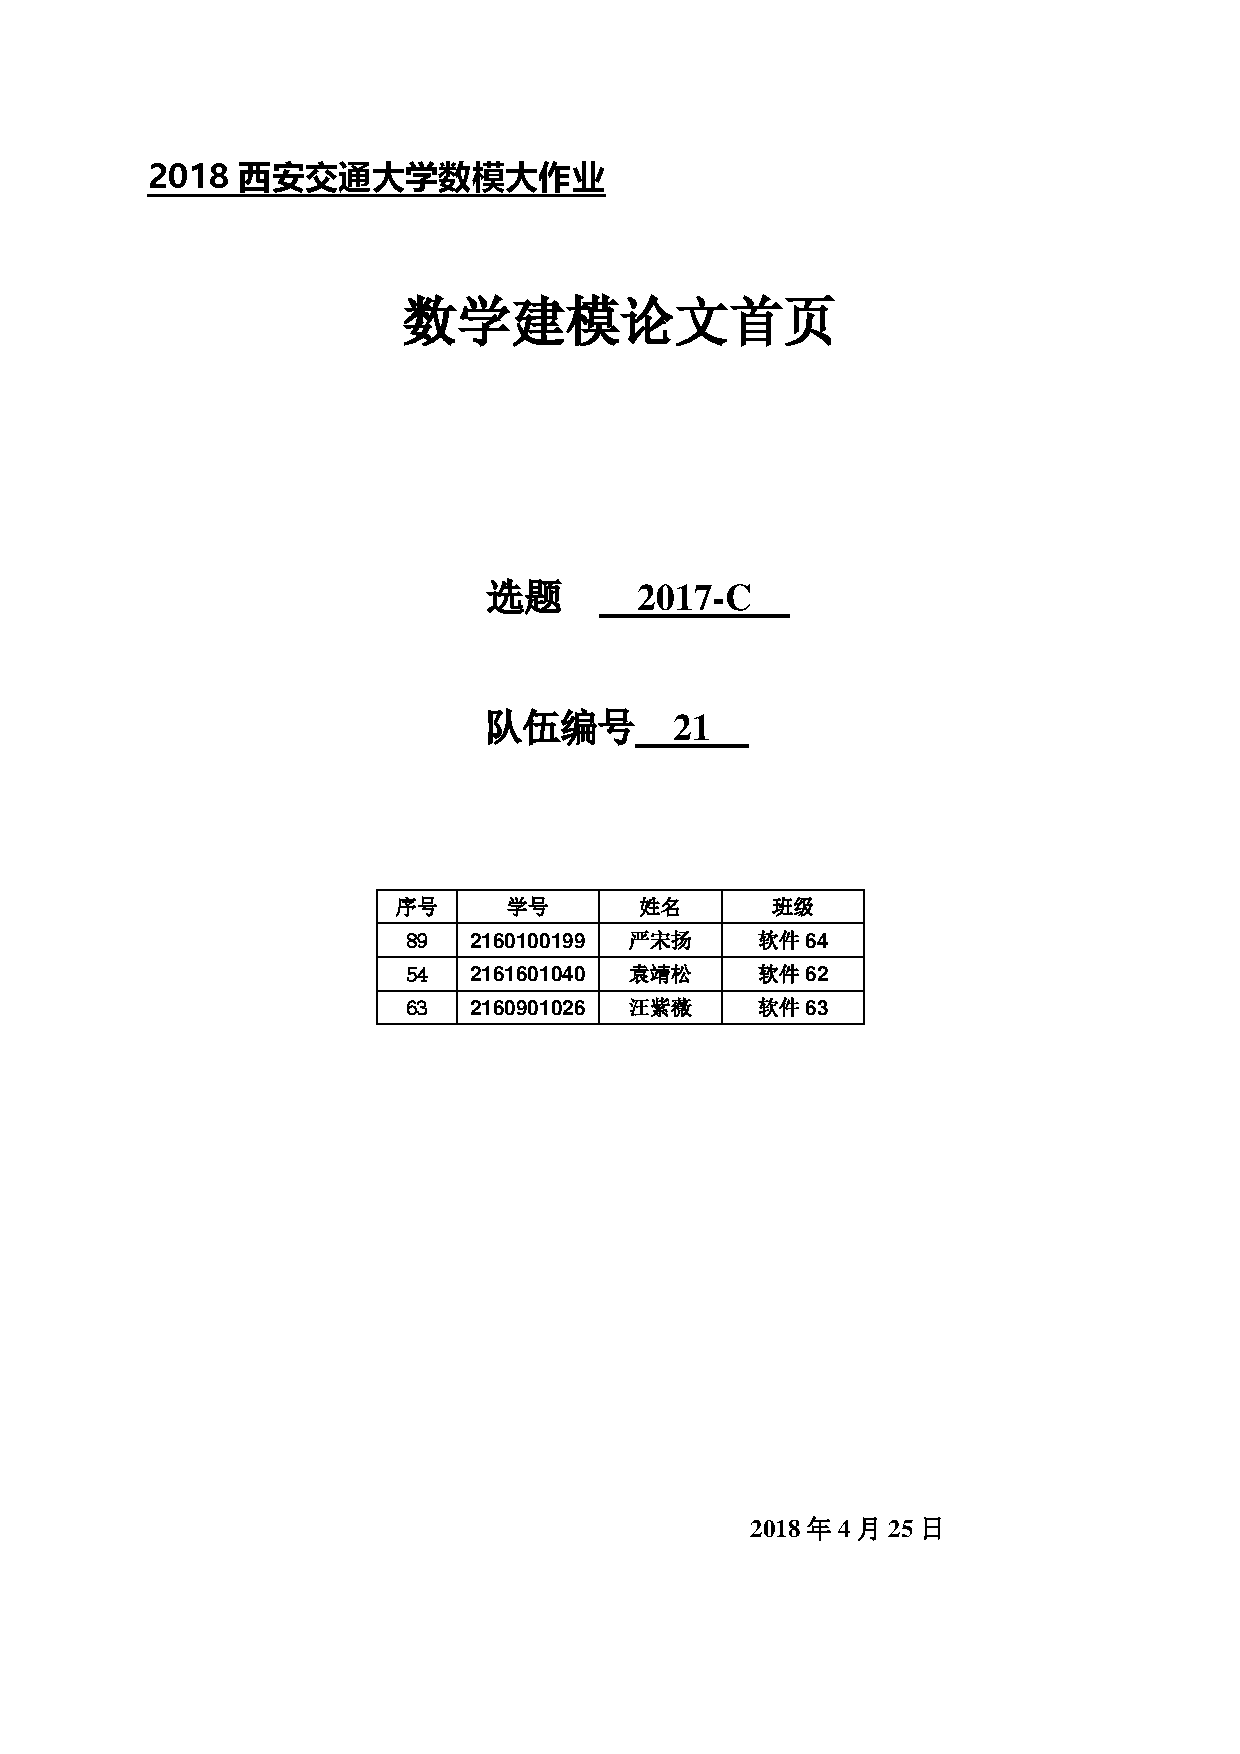
\includegraphics[width=\textwidth]{cover.pdf}
\end{titlepage}

\maketitle

\begin{abstract}

为了更精确地通过溶液的颜色读数确定物质的浓度,本文研究了题目提供的各物质颜色读数与物质浓度的关系。

对于问题一各物质,首先对原始数据进行处理,引入灰度值为数据降维,并计算各参数之间的相关系数与各参数对于物质浓度的相关系数。
使用灰度值分别对组胺浓度和溴酸钾浓度进行回归分析,得到结果为$\text{组胺浓度}=-3.034\times \text{灰度}+327.4$,
$\text{溴酸钾浓度}=-5.291\times \text{灰度}+731.6$。
对于工业碱,直接使用灰度进行回归分析效果不显著,去除掉数据中的离群点(浓度为0的点)后,回归效果显著,但只适用于浓度在$[7,12]$区间的情况,
结果为$\text{工业碱浓度}=-0.03599\times \text{灰度}+12.93$。
对于硫酸铝钾,首先通过分析其数据特征建立通过RGB平均数数值判定其浓度是否小于0.5ppm的判定模型。
由于H、S随浓度的变化符合酶促反应速率特点,引入描述酶促反应的指数增长模型和快速平衡模型,
得到的最优结果为$\text{硫酸铝钾浓度}=(0.38H-28.35)\div(510-5H)$。
对于奶中尿素,使用参数B进行一维线性回归,得到结果为$\text{奶中尿素浓度}=-129.7B+ 15490$。

设计准确度、稳定度、区分度、吻合度四个指标,建立综合评价模型以进行数据质量评价。
其中吻合度为HS测量值与计算值的相差程度,由于吻合度的区分度太小,故将其从模型中舍去。
准确度用所测数据的组数来衡量,稳定度用同物质同浓度下数据变异系数来衡量,区分度用同物质异浓度的数据离散度来衡量。
最终得出的数据质量评价得分为:组胺0.4236,溴酸钾0.5538,工业碱0.4977,硫酸铝钾0.5014,奶中尿素0.0888。

对于问题二,通过R、G、B计算出H、S的计算值与测量值对比,发现数据表中H、S两列位置恰好相反,故将其修正。
先利用数据质量的综合评价模型检验其数据质量,发现质量良好,可用于分析。
绘制折线图,发现灰度和参数G与浓度有较为明显的线性关系,尝试建立一元线性回归模型,结果效果不佳。
使用指数增长模型对灰度与浓度进行回归分析,得到回归系数的置信区间包含零点,无法采纳。
再使用快速平衡模型对参数S和浓度进行分析,得到的结果较好,可以适用于实际:$\text{二氧化硫浓度}=(124.1S-359.45)\div(142.01-S)$。

对于问题三,分别说明数据量和数据维度对于模型质量的影响。
通过对比数据量较少的溴酸钾和数据量较多的硫酸铝钾,得出数据量越大模型的精度和普适性越高,但也会加大数据处理难度的结论。
通过讨论RGB模型和HSV模型的转换关系,对比问题一、二中各项回归分析,
得出结论为:数据维度多则包含信息越多,但不一定能得到更准确的模型,在使用维度较低的数据建成的模型可用的情况下,则没有必要对更多维的数据进行讨论。

\keywords{回归分析\quad  酶促反应\quad  数码照片比色法\quad  灰度\quad   RGB和HSV\quad }
\end{abstract}
\section{符号说明}

\begin{table}[H]
    \centering
    \caption{符号说明}
    %\label{my-label}
    \begin{tabular}{@{}cc@{}}
    \toprule
    符号       & 意义         \\ \midrule
    $R$      & RGB模型的红色强度        \\
    $G$      & RGB模型的绿色强度       \\
    $B$      & RGB模型的蓝色强度  \\
    $H$      & 色调       \\
    $S$      & 饱和度  \\
    $c$   & 浓度   \\
    $Gr$   & 灰度      \\ \bottomrule
    \end{tabular}
\end{table}
\section{问题假设}
1.假设R,G,B,H,S的数据都是实际测量未受主观影响的

2.测量的物质中杂质或其他成分对颜色没有影响


\section{问题重述}
比色法是目前常用的一种检测物质浓度的方法,即把待测物质制备成溶液后滴在特定的白色试纸表面,
等其充分反应以后获得一张有颜色的试纸,再把该颜色试纸与一个标准比色卡进行对比,就可以确定待测物质的浓度档位。
现在我们需要给出一个精确的方法通过测量颜色读数从而获得待测物质的浓度。
\subsection{问题一}
(1)通过附件1所给出的5组数据确定各物质颜色读数和物质浓度的关系

(2)给出评价标准并评价一直数据的精准程度

\subsection{问题二}
(1)通过附件2所给出的模型,建立颜色读数和浓度间的模型

(2)通过(1)中建立的模型进行误差分析

\subsection{问题三}
(1)探讨数据量对模型的影响

(2)探讨颜色维度对模型的影响

\section{问题假设}
假设R,G,B,H,S的数据都是实际测量未受主管影响的
测量的物质中杂质或其他成分对颜色没有影响

\section{符号说明}

\section{问题分析}
\subsection{问题一分析}
问题一是对于某种物质,输入其不同的颜色维度,得到对应的浓度值。附件1中的数据分别给了物质名称,
物质浓度,R, G, B, H, S 这几个维度的量,颜色读数有两套独立的规则体系,分别是RGB体系与HSV体系
,两套体系之间可以互相转换。所以,我们先利用主成分分析法,找出对于不同物质各个属性值之间的相关性,
对于相关性大的,我们可以采取降维处理的方式,减少变量个数,简化模型,对于相关性小的,我们则必须利用不同的属性,
建立不同的模型。对于建立的模型,我们采用 $R^2$, $RMSE$两个指标去衡量模型优劣,同时采用参数的置信区间
筛选参数,选择模型是否使用。
对于数据评价标准,我们建立了衡量数据评价的模型,利用数据评价模型,我们评价不同物质的数据质量。

\subsection{问题二分析}
问题二是对于附件二所给的数据建立合适的模型。对于附件二所给的数据,经过计算,发现所给的数据有一定的误差,
进行数据处理之后,建立灰度与浓度的一元线性回归模型。发现模型效果不好后,考虑建立非线性模型,尝试建立指数增长模型
和快速增长模型,同样采用$R^2$,$RMSE$这两个指标评价模型建立的效果,选取适当的模型。

\subsection{问题三分析}
问题三是对于不同的数据量和颜色维度对数学模型的影响。所以我们选择了数据量过少的溴酸钾与其他物质进行
对比,比较数据量的多少会对数学模型的精度产生的影响。同时,对于同一个物质,我们比较了不同维度下建立的
数学模型之间准确度,从而比较维度是否会对建立的数学模型精度产生影响。

\section{问题一的分析求解}
\subsection{数据处理}
        因为RGB值之间具有很强的自相关性,无法对RGB三个变量建立多元回归方程,考虑到灰度$^{\cite{gr}}$处理是常见的图像处理手段,
        所以先将对应的RGB值转化成灰度。根据灰度计算公式
        $$Gr = 0.2989R + 0.587G + 0.114B$$
        可以得到各物质在不同浓度下的灰度值。
        继续尝试计算RGB的算数平均数和几何平均数,探索浓度是否与RGB的算术平均数和几何平均数有关。
  %      \begin{table}
  %      \begin{tabular}{|c|c|c|c|c|}
  %          \hline
  %          物质 & 浓度 & 灰度 & RGB算术平均数 & RGB几何平均数\\
  %          \hline
  %          \multirow{5}*{组胺} & 0 & 108.18 & 99 & 95.86 \\
  %          & 12.5 & 102.27 & 94.8 & 91.99 \\
  %          &25 & 100.947 & 93.34 & 89.32 \\
  %          &50 & 91.45 & 83.5 & 77.76 \\
  %          &100 & 75.00 & 70.15 & 63.51 \\
  %          \hline
  %          \multirow{5}*{溴酸钾} & 0 & 140.61&138&137.83 \\
  %          &12.5 & 133.35 & 123.33 & 120.11 \\
  %          &25 & 128.89 & 113.5 & 111.34 \\ 
  %          &50 & 126.88 & 110.83 & 103.13 \\
  %          &100 & 122.22 & 95 & 51.30 \\
  %          \hline
  %           \multirow{7}*{工业碱} & 0 & 140.15 & 142 & 141.76 \\
  %          & 7.34 & 139.09 & 141.67 & 141.40 \\
  %          & 8.14 & 140.34 & 142 & 141.81 \\ 
  %          & 8.74 & 129.95 & 137 & 136.23 \\
  %          & 9.19 & 103.53 & 121.33 & 117.32\\
  %          & 10.18 & 62.39 & 89 & 68.21\\
  %          & 11.8 & 41.45 & 63.67 & 37.16\\
  %          \hline
  %            \multirow{6}*{硫酸铝钾} & 0 & 117.64 & 114.61& 114.28 \\
  %          & 0.5 & 101.87 & 105.44 & 98.76\\
  %          & 1 & 100.36 & 104.78 & 96.38\\ 
  %          & 1.5 & 98.89 & 104.95 & 93.91\\
  %          & 2 & 92.04 & 101.17 & 85.49\\
  %          & 5 & 93.45 & 100.83 & 86.75\\
  %          \hline
  %             \multirow{6}*{奶中尿素} & 0 & 134.99 & 131.89 & 131.64 \\
  %          &500 & 135.48 & 131.11 & 130.69 \\
  %          &1000 & 133.48 & 128 & 127.34\\ 
  %          &1500 & 133.14 & 127.11 & 126.39\\
  %          &2000 & 134.14 & 127.56 & 126.64\\
  %          \hline
  %    \end{tabular}
  %\end{table}
   根据数据处理结果,可以看到对于组胺和溴酸钾而言,灰度和其浓度之间有着明显的负相关,所以可以使用一元线性回归方程对其拟合,
   而工业碱,硫酸铝钾和奶中尿素对于灰度的相关性则不强,说明不能单纯使用灰度进行拟合,应该重新使用新的模型进行拟合。
\subsection {对组胺浓度与颜色读数间关系的分析}

    将所给的数据画出对应的RGB折线图如图~\ref{ZA_RGB_C}所示。

    \quickF{0.6}{ZA_RGB_C.png}{组胺浓度关于RGB的折线图}{ZA_RGB_C}

    根据图~\ref{ZA_RGB_C},可以看到R,G,B均与组胺浓度$c$有着明显的线性关系,且随着组胺浓度增加,均有着
    减少的趋势,并且三者的变化范围较大,可以看出较大的差距。

    显然组胺浓度与与RGB有着强烈的负相关性,而RGB属性之间又有着自相关性,进一步计算RGB之间的自相关性系数
    如表~\ref{组胺各颜色参数相关系数}所示。
      \begin{table}[H]
        \caption{组胺各颜色参数间的自相关系数}
        \label{组胺各属性相关系数}
        \centering
        \begin{tabular}{|c|c|c|c|c|c|c|}
        \hline
            \diagbox{颜色参数}{颜色参数} & B & G & R & H & S & Gr \\
            \hline
            B & 1    & 0.97 & 0.87  & 0.95 & -0.99 & \null \\
            \hline
            G & 0.97 & 1    & 0.945 & 0.98 & -0.96 & \null \\
            \hline
            R & 0.87 & 0.94 &   1   & 0.89 & -0.84 & \null \\
            \hline
            H & 0.95 & 0.98 & 0.89  &   1  & -0.94 & 0.97  \\
            \hline
            S & -.99 & -0.96& -0.84 & -0.94&   1   & -0.96 \\
            \hline
        \end{tabular}
    \end{table}

    从表~\ref{组胺各属性相关系数}可以看出,B,G,R均有着较大的相关性,所以如果直接使用三元变量进行拟合
    可能不会得到较好的结果,所以可以使用灰度作为自变量,将每组RGB值转化为灰度,进行一元线性拟合。

    根据所给的两组数据,我们可以看到两组数据的偏差范围不大,所以可以使用两组数据的平均数进行数据处理。
    进一步计算R,G,B,H,S,Gr,RGB算数平均数,RGB几何平均数与组胺浓度的相关系数,得到对应的相关系数如表~\ref{ZuAnCov}所示。
    \begin{table}[H]
        \centering
        \caption{各颜色参数与组胺浓度的相关系数}
        \label{ZuAnCov}
        \begin{tabular}{@{}ccccccccc@{}}
        \toprule
        颜色参数 & R       & G      & B       & H       & S       &  Gr    & RGB算术平均数 & RGB几何平均数 \\ \midrule
        相关系数 & -0.9313 & -0.997 & -0.9724 & -0.9778 & 0.96272 & -0.996 & -0.995   & -0.993   \\ \bottomrule
        \end{tabular}
        \end{table}
         
    由表~\ref{ZuAnCov}可以看到,灰度与组胺浓度的相关性系数绝对值较接近1,有着强烈的相关性,所以我们
    可以直接使用灰度作为自变量对浓度进行一元线性回归,这样一方面简化了模型,
    另一方面并没有过多地丢失精度。

    绘制组胺浓度与灰度折线图如图~\ref{ZA_Gr_C}所示。

    \quickF{0.6}{ZA_Gr_C.png}{组胺浓度关于灰度的折线图}{ZA_Gr_C}

    根据所绘制的图~\ref{ZA_Gr_C},可以看出灰度与组胺浓度近似服从一元线性模型,建立线性回归模型
    $$ y = p_1 \times x + p_2$$
    其中 $p_{1}, p_{2}$为回归系数,$x$为灰度,$y$为组胺浓度。利用 Matlab 软件进行求解得到的回归系数估计值及置信区间,检验统计量 $R^2, RMSE $结果如表~\ref{ZuAnLinear}所示。

    \begin{table}[H]
        \centering
        \caption{一元拟合的参数结果}
        \label{ZuAnLinear}
        \begin{tabular}{@{}ccc@{}}
        \toprule
        参数         & 参数估计值      & 参数置信区间                  \\ \midrule
        $p_1$      & -3.034     & {[}-3.248, -2.82{]}     \\
        $p_2$      & 327.4      & {[}306.9, 348{]}     \\
        \hline
        \multicolumn{3}{c}{$R^2$ = 0.9926 $RMSE$ = 3.404} \\ \bottomrule
        \end{tabular}
        \end{table}

    结果分析: 从表~\ref{ZuAnLinear}可以看出 $R^2$ 近似为1,$RMSE$的值为3.404,且每个回归系数的置信区间没有包含零点,说明灰度值对浓度影响是显著的,
    所以模型在整体上是合理可用的。说明组胺的浓度可以通过颜色读数来确定,其预测的方程为
    $$c = -3.034Gr + 327.4 $$
    
    因为H,S与组胺的浓度的相关性系数也较大,也可以尝试用以H,S为自变量。进行二元函数线性回归拟合,以求得到更为精确的模型。
    建立二元函数拟合方程为
    $$ z = p_{00} + p_{10} \times x + p_{01} \times y$$
    其中,$x$ 为 H, $y$ 为 S,$z$为组胺浓度,$p_{00},p_{10},p_{01}$ 为回归系数,利用 Matlab 软件进行求解得到回归系数估计值及置信区间,
    检验统计量 $R^2, RMSE $结果如表~\ref{ZuAn2Dim}所示。

    \begin{table}[H]
        \centering
        \caption{二元拟合的参数结果}
        \label{ZuAn2Dim}
        \begin{tabular}{@{}lcc@{}}
        \toprule
        参数       & 参数估计值  & 参数置信区间                       \\ \midrule
        $p_{00}$ & 60.72  & {[}-100.6, 222{]}    \\
        $p_{10}$ & -5.5   & {[}-9.439, -1.561{]} \\
        $p_{01}$ & 0.5614 & {[}-0.1248, 1.248{]} \\
        \hline
        \multicolumn{3}{c}{$R^2$ = 0.914 $RMSE$ =7.147}  \\ \bottomrule
        \end{tabular}
        \end{table}

    结果分析: 从表~\ref{ZuAn2Dim}中可以看出 $R^2$ 近似为1,$RMSE$的值为7.147,但是注意到$p_{00}$的置信区间和$p_{01}$的置信区间含有零点,
    说明这两个参数不是很显著,所以这个模型不在这里适用。

\subsection{对溴酸钾浓度与颜色读数间关系的分析}

    将所给的数据画出对应的RGB折线图,如图~\ref{XSJ_RGB_C}所示。

    \quickF{0.6}{XSJ_RGB_C.png}{溴酸钾浓度关于RGB的折线图}{XSJ_RGB_C}

    从图中可以看到,随着溴酸钾浓度的增加,G,R所对应的两条折线趋势基本趋于平缓, 大概可以判断溴酸钾浓度与G,R这两个维度没有较大的联系,
    进一步计算RGB之间的自相关性系数如表~\ref{溴酸钾相关性系数图}所示。
    \begin{table}[H]
        \centering
        \caption{溴酸钾各颜色参数的自相关性系数}
        \label{溴酸钾相关性系数图}
        \begin{tabular}{|c|c|c|c|c|c|c|}
            \hline
            \diagbox{颜色参数}{颜色参数} & B & G & R & H & S & Gr \\
            \hline
            B & 1 & 0.89 & 0.07 & -0.85 & -0.99 & \null \\
            \hline
            G & 0.89 & 1 & 0.46 & -0.87 & -0.89 & \null \\
            \hline
            R & 0.07 & 0.46 & 1 & -0.24 & -0.05 & \null \\
            \hline
            H & -0.85 & -0.87 & -0.24 & 1 & 0.84 & -0.88 \\
            \hline
            S & -0.99 & -0.89 & -0.05 & 0.84 & 1 & -0.97 \\
            \hline
        \end{tabular}
    \end{table}

    根据图~\ref{溴酸钾相关性系数图}可以看到,R与其他变量相关性系数较差,
    但B与G相关性系数较强,所以不能直接使用三元变量进行多元函数拟合,可以
    考虑使用灰度进行一元线性回归拟合。

    对于所给的两组数据,两组数据的极差很小,所以可以直接使用两组数据的平均数进行数据分析,分别计算R,G,B,H,S,灰度,RGB算术平均数,
    RGB几何平均数与溴酸钾浓度的相关系数,得到对应的相关系数如表~\ref{多变量与溴酸钾浓度}所示。

    \begin{table}[H]
        \centering
        \caption{各颜色参数与溴酸钾浓度的相关系数}
        \label{多变量与溴酸钾浓度}
        \begin{tabular}{@{}ccccccccc@{}}
        \toprule
        参数 & R     & G     & B     & H    & S    & 灰度    & RGB算数平均数 & RGB几何平均数 \\ \midrule
        相关系数 & -0.16 & -0.87 & -0.96 & 0.69 & 0.95 & -0.95 & -0.96    & -0.96    \\ \bottomrule
        \end{tabular}
        \end{table}

    由表~\ref{多变量与溴酸钾浓度}中计算的数据,可以看到灰度与浓度的相关性系数绝对值接近1,有着一定的相关性,
    所以我们可以直接使用灰度作为自变量对溴酸钾浓度进行一元的线性回归。这样,一方面简化了模型的复杂度,另一方面并没有过多的丢失精度。

    绘制溴酸钾浓度与灰度折线图如图~\ref{XSJ_Gr_C}所示。

    \quickF{0.6}{XSJ_Gr_C.png}{溴酸钾浓度关于灰度的折线图}{XSJ_Gr_C}

    从图\ref{XSJ_Gr_C}可以看出,灰度与溴酸钾浓度点近似服从线性分布。 以灰度为自变量建立线性回归模型
    $$ y = p_1 \times x + p_2$$
    其中 $p_{1},p_{2}$为回归系数, $x$为灰度,$y$为溴酸钾浓度。利用 Matlab 软件进行求解得到回归系数估计值及置信区间,
    检验统计量 $R^2, RMSE $结果如表~\ref{溴酸钾一元拟合}所示。

    \begin{table}[H]
        \centering
        \caption{以灰度为自变量一元拟合结果}
        \label{溴酸钾一元拟合}
        \begin{tabular}{@{}ccc@{}}
        \toprule
        参数        & 参数估计值      & 参数置信区间                   \\ \midrule
        $p_1$     & -5.291     & {[}-6.765, -3.817{]}     \\
        $p_2$     & 731.6      & {[}538, 925.2{]}         \\
        \hline
        \multicolumn{3}{c}{$R^2$ = 0.8954 $RMSE$ = 12.78} \\ \bottomrule
        \end{tabular}
        \end{table}
    从表~\ref{溴酸钾一元拟合}可以看到$R^2$近似为1,$RMSE$值为12.78,并且两个参数的置信区间并没有包含零点,说明灰度值对溴酸钾浓度影响是显著的,
    因此模型在整体上是合理可用的。说明溴酸钾的浓度可以通过颜色读数来确定,其预测的方程为
    $$ c = -5.291Gr + 731.6 $$ 

    根据表\ref{多变量与溴酸钾浓度}可以看到RGB的几何平均数与溴酸钾浓度也有较强的关系,也可以尝试采用以RGB的几何平均数为自变量对浓度进行一元线性回归。
    建立一元线性回归方程为
     $$ y = p_1 \times x + p_2$$
    其中 $x$为RGB几何平均数,$y$为溴酸钾浓度,$p_1, p_2$为回归系数。利用 Matlab 软件进行求解得到的回归系数估计值及置信区间,检验统计量 $R^2, RMSE $结果如表~\ref{RGB拟合}

    \begin{table}[H]
        \centering
        \caption{以RGB几何平均数为自变量一元拟合结果}
        \label{RGB拟合}
        \begin{tabular}{@{}ccc@{}}
        \toprule
        参数        & 参数估计值     & 参数置信区间                  \\ \midrule
        $p_1$     & -1.197    & {[}-1.367, -1.026{]}    \\
        $p_2$     & 162.9     & {[}144.3, 181.4{]}      \\
        \hline
        \multicolumn{3}{c}{$R^2$ = 0.9704 $RMSE$ = 6.8} \\ \bottomrule
        \end{tabular}
        \end{table}

    从表~\ref{RGB拟合}可以看到$R^2$ 近似值为1,$RMSE$值为6.8,并且两个参数的置信区间并没有包含零点,说明RGB的几何平均数对溴酸钾浓度影响是显著的,
    因此模型在整体上是合理可用的。说明溴酸钾的浓度也可以通过颜色读数来确定,其预测的方程为
    $$ c = -1.197 \hat{RGB} + 162.9 $$

    根据表~\ref{溴酸钾一元拟合}和表~\ref{RGB拟合}结果,可以看出使用RGB的几何平均数拟合效果较好,即溴酸钾的浓度可以通过
    RGB集合平均数得出,预测的方程为
    $$ c = -1.197 \hat{RGB} + 162.9 $$

    同时根据上面的表\ref{溴酸钾相关性系数图},发现H,S与溴酸钾浓度的相关系数也很大,所以以H,S为自变量进行了多元函数的拟合分析,
    建立二元回归方程 为
    $$ z = p_{00} + p_{10} \times x + p_{01} \times y$$
    其中,$x$ 为$H$, $y$ 为 $S$,$z$为溴酸钾浓度,$p_{00},p_{10},p_{01}$ 代表回归系数,利用 Matlab 软件进行求解得到的回归系数估计值及置信区间,
    检验统计量 $R^2, RMSE $结果如表~\ref{二元拟合结果}所示。

    \begin{table}[H]
        \centering
        \caption{以H,S为自变量二元拟合结果}
        \label{二元拟合结果}
        \begin{tabular}{@{}ccc@{}}
        \toprule
        参数         & 参数估计值     & 参数置信区间                  \\ \midrule
        $p_{00}$     & 155.8     & {[}-29.68, 341.2{]}     \\
        $p_{10}$     & -7.897    & {[}-15.92, 0.1276{]}    \\
        $p_{01}$     & 0.6479    & {[}0.4536, 0.8423{]}    \\
        \hline
        \multicolumn{3}{c}{$R^2$ = 0.9478 $RMSE$ =9.653} \\ \bottomrule
        \end{tabular}
        \end{table}

    结果分析: 从表~\ref{二元拟合结果}可以看出 $R^2$ 近似为1,$RMSE$的值为9.653,但是注意到$p_{00}$的置信区间和$p_{01}$的置信区间含有零点,
    说明这个这个参数不是很显著,所以这个模型不能在这里使用。

\subsection{对工业碱浓度与颜色读数间关系的分析}
    通过分析原始数据,发现浓度为0的点和浓度为7.34的点所对应的RGBHS值大体相等,但由于浓度为0的点与其他浓度测量值偏离较大,所以可以判断浓度为0的点不是一个有效数据,
    故排除浓度为0的点进行分析。将浓度为0的点剔除后,绘制对应的RGB折线图如图~\ref{GYJ_RGB_C_no0}所示。

    \quickF{0.6}{GYJ_RGB_C_no0.png}{工业碱浓度去除零点后关于RGB的折线图}{GYJ_RGB_C_no0}

    由图~\ref{GYJ_RGB_C_no0}可以发现,RGB 三条曲线所对应的趋势基本相同相同,变化不大,
    判断RGB之间可能有较大的线性相关性。进一步计算他们之间的相关性系数如表~\ref{工业碱浓度相关系数图}所示。

    \begin{table}[H]
        \centering
        \label{工业碱浓度相关系数图}
        \caption{工业碱各个参数间的自相关系数}
            \begin{tabular}{|c|c|c|c|c|c|c|}
                \hline
                \diagbox{参数}{参数} & B & G & R & H & S & Gr \\
                \hline
                B & 1 & 0.83 & 0.86 & -0.71 & -0.83 & \null \\
                \hline
                G & 0.83 & 1 & 0.87 & -0.97 & -0.99 & \null \\
                \hline
                R & 0.86 & 0.87 & 1 & -0.84 & -0.88 & \null \\
                \hline
                H & -0.71 & -0.97 & -0.84 & 1 & 0.97 & -0.96 \\
                \hline
                S & -0.83 & -0.99 & -0.88 & 0.97 & 1 & -0.99 \\
                \hline
            \end{tabular}
        \end{table}
   
    根据表~\ref{工业碱浓度相关系数图}可以看到 RGB 之间相关性系数较大,
    所以不能直接使用三元变量进行线性回归拟合,可以尝试使用灰度进行一元线性回归拟合。

    绘制工业碱浓度与灰度折线图如图~\ref{GYJ_Gr_C}所示。

    \quickF{0.6}{GYJ_Gr_C.png}{工业碱浓度关于灰度的折线图}{GYJ_Gr_C}

    从图~\ref{GYJ_Gr_C}可以看到,在去除掉浓度为0的点后,工业碱浓度与灰度近似服从一元线性模型,
    所以可以使用灰度进行一元回归分析,建立一元线性回归模型
    $$ y = p_1 \times x + p_2 $$
    其中,$x$为灰度,$y$为工业碱浓度,$p_1, p_2$为回归系数。利用 Matlab 软件进行求解得到的回归系数估计值及置信区间,
    检验统计量$R^2, RMSE $结果如下 

    \begin{table}[H]
        \centering
        \caption{以灰度为自变量一元拟合结果}
        \label{灰度工业碱一元拟合}
        \begin{tabular}{@{}ccc@{}}
        \toprule
        参数       & 参数估计值      & 参数置信区间                     \\ \midrule
        $p_1$    & -0.03599   & {[}-0.05097, -0.02101{]}   \\
        $p_2$    & 12.93      & {[}11.29, 14.58{]}         \\
        \hline
        \multicolumn{3}{c}{$R^2$ = 0.9175 $RMSE$ = 0.5079} \\ \bottomrule
        \end{tabular}
        \end{table}

    结果分析: 从表~\ref{灰度工业碱一元拟合}可以看出 $R^2$ 近似为1,$RMSE$的值为0.5079,且每个回归系数的置信区间没有包含零点,
    说明灰度值对浓度影响是显著的,所以模型在整体上是合理可用的。说明工业碱溶液的浓度可以通过颜色读数来确定,其预测方程为:
        $$c = -0.03599 Gr + 12.93 $$
    注意:由于所给的数据量过少,且浓度变化范围主要集中在 $7 \sim 12$之间,所以我们根据灰度来预测时灰度的取值范围也应在 $40 \sim 140$
    之间。
\subsection{硫酸铝钾颜色与浓度的关系}

    将硫酸铝钾的R,G,B,H,S数据按浓度分组,并计算每组平均值,RGB算术平均数和几何平均数。
    取计算所得平均值绘制 R, G, B,灰度与浓度的折线图如图~\ref{LSLJ_RGBGr_C}所示。

    \quickF{0.6}{LSLJ_RGBGr_C.png}{硫酸铝钾浓度关于RGB和灰度的折线图}{LSLJ_RGBGr_C}
    
    观察图~\ref{LSLJ_RGBGr_C}发现,随着硫酸铝钾浓度的增加, R, G, B的值没有明显的变化趋势,只在浓度为0和浓度为0.5$ppm$及以上有明显的差异。因此分为保留浓度为0的数据和除去浓度为0的数据两种情况分别分析。
    计算灰度和浓度的相关性如表~\ref{硫酸铝钾浓度和灰度}所示。
    \begin{table}[H]
      \centering
      \caption{灰度和硫酸铝钾浓度的相关性}
      \label{硫酸铝钾浓度和灰度}
      \begin{tabular}{@{}ccc@{}}
      \toprule
      浓度 & 包括0     & 不包括0    \\ \midrule
      相关系数 & -0.6778 & -0.7195 \\ \bottomrule
      \end{tabular}
    \end{table}
    
    观察表~\ref{硫酸铝钾浓度和灰度}发现灰度和浓度的相关性不强。无法建立有关模型。
    
    而由于浓度为0的数据和浓度为0.5ppm及以上的数据之间有较为明显的差异,若只需要粗略估计浓度,可以建立一个简略的颜色与浓度的模型。
    $$ c<0.5 \text{ ppm}, \text{if } aver(RGB)>105 $$
    式中 R, G, B的取值范围均在0到255之间,$aver(RGB)$为RGB三个数的数值的算术平均数。
    
    绘制H, S和浓度的折线图如图~\ref{LSLJ_HS_C}所示。

    \quickF{0.6}{LSLJ_HS_C.png}{硫酸铝钾浓度关于HS的折线图}{LSLJ_HS_C}
    
    发现随着浓度的增加,H, S两类数据的变化规律类似,均为在浓度低是快速增加,而浓度高时缓慢增加。
    由此联想到酶促反应$^{\cite{mm}}$$^{\cite{exp}}$中反应速度和底物浓度之间的关系。对于酶促反应的性质,满足的模型有两个:
    
    指数增长模型:$$y=\beta_0(1-e^{-\beta_1x})$$

    $Michaelis-Menten$模型(米-曼式模型,也叫快速平衡模型):
    $$y=\frac{\beta_0x}{\beta_1+x}$$
    
    首先用指数增长模型对该组数据进行回归分析,其中 H 值和 S 值作为自变量,硫酸铝钾浓度作为因变量,得到结果:
    
    \begin{table}[H]
      \centering
      \caption{硫酸铝钾浓度和H值指数增长模型回归分析结果}
      \label{硫酸铝钾浓度和H值指数}
      \begin{tabular}{@{}ccc@{}}
      \toprule
      参数        & 参数估计值      & 参数置信区间                   \\ \midrule
      $\beta_0$     & -3.065e-12     & {[}-2.316e-10, 2.255e-10{]}     \\
      $\beta_1$     & -0.2703   & {[}-1.006, 0.4653{]}    \\
      \hline
      \multicolumn{3}{c}{$R^2$ = 0.3548   $RMSE$ = 1.598} \\ \bottomrule
      \end{tabular}
    \end{table}
    
    从表~\ref{硫酸铝钾浓度和H值指数}中可以看到,$R^2$为0.3548,且参数的置信区间跨零点,所以该模型不可用。

    \begin{table}[H]
        \centering
        \caption{硫酸铝钾浓度和S值指数增长模型回归分析结果}
        \label{硫酸铝钾浓度和S值指数}
        \begin{tabular}{@{}ccc@{}}
        \toprule
        参数        & 参数估计值      & 参数置信区间                   \\ \midrule
        $\beta_0$     & -0.01464     & {[}-0.1857, 0.1564{]}     \\
        $\beta_1$     & -0.02784    & {[}-0.0898, 0.03411{]}    \\
        \hline
        \multicolumn{3}{c}{$R^2$ = 0.551   $RMSE$ = 1.333} \\ \bottomrule
        \end{tabular}
      \end{table}
    
      从表~\ref{硫酸铝钾浓度和S值指数}中可以看到,$R^2$为0.551,仅稍好于比 H 值回归模型,且参数的置信区间跨零点,模型不可用。

    
    然后选择$Michaelis-Menten$模型对该组数据进行回归分析。取硫酸铝钾浓度作为自变量,H值和S值作为因变量,带入模型:
    
    $$y=\frac{\beta_0x}{\beta_1+x}+\beta_2$$
    硫酸铝钾浓度和H值的拟合结果如表~\ref{硫酸铝钾浓度和H值M-M}所示。
    \begin{table}[H]
      \centering
      \caption{H 值为自变量的$Michaelis-Menten$模型拟合结果}
      \label{硫酸铝钾浓度和H值M-M}
      \begin{tabular}{@{}ccc@{}}
      \toprule
      参数        & 参数估计值      & 参数置信区间                   \\ \midrule
      $\beta_0$     & 27.33     & {[}22.96, 31.7{]}     \\
      $\beta_1$     & 0.07594   & {[}-0.03905, 0.1909{]}    \\
      $\beta_2$     & 74.67     & {[}71.33, 78{]}         \\
      \hline
      \multicolumn{3}{c}{$R^2$ = 0.9941   $RMSE$ = 1.048} \\ \bottomrule
      \end{tabular}
    \end{table}
    
    从表~\ref{硫酸铝钾浓度和H值M-M}中可以看到,$R^2$接近1,$RMSE$的值为1.048,虽然参数$\beta_1$的置信区间包括零点,
    但因为$\beta_1$为常数项,不是总体参数,模型可用。

    同理,计算硫酸铝钾浓度和S值的拟合结果如表~\ref{硫酸铝钾浓度和S值M-M}所示。
    
    \begin{table}[H]
      \centering
      \caption{S 值为自变量的$Michaelis-Menten$模型拟合结果}
      \label{硫酸铝钾浓度和S值M-M}
      \begin{tabular}{@{}ccc@{}}
      \toprule
      参数        & 参数估计值      & 参数置信区间                   \\ \midrule
      $\beta_1$     & 160.1     & {[}118.6, 201.7{]}     \\
      $\beta_2$     & 0.2812   & {[}-0.02671, 0.5891{]}    \\
      $\beta_3$     & 42.5     & {[}13.38, 71.63{]}         \\
      \hline
      \multicolumn{3}{c}{$R^2$ = 0.9842   $RMSE$ = 9.159} \\ \bottomrule
      \end{tabular}
    \end{table}
    
    从表~\ref{硫酸铝钾浓度和S值M-M}中可以看到,$R^2$接近1,$RMSE$的值为9.159,相比浓度和 H 值的回归结果较差。
    选择硫酸铝钾浓度和 H 值的建立的$Michealis-Menten$模型得到硫酸铝钾颜色和浓度的模型:
    $$c=\frac{0.38H-28.35}{510-5H}$$
    
    \subsection{奶中尿素颜色与浓度的关系}
    计算奶中尿素浓度和个颜色参数的相关性如表~\ref{奶中尿素浓度相关性}所示。
    
    \begin{table}[H]
      \centering
      \caption{奶中尿素浓度和各颜色参数的相关性}
      \label{奶中尿素浓度相关性}
      \begin{tabular}{@{}ccccccccc@{}}
      \toprule
      参数 & R  & G & B & H & S&灰度 & RGB算术平均数 & RGB几何平均数\\ \midrule
      相关系数 & -0.4369 & -0.3451  &-0.9603 & 0.6484 &0.9433 & -0.6165 & -0.8551 & -0.8785\\ \bottomrule
      \end{tabular}
    \end{table}
    
    观察表~\ref{奶中尿素浓度相关性}发现B的值和浓度的相关性较强而与灰度的相关性较差,
    以颜色参数B为自变量,奶中尿素浓度为因变量建立一元线性回归模型
    $$ y = p_1 \times x + p_2$$
    其中$x$为颜色参数B,$y$为奶中尿素浓度,$p_1$,$p_2$为回归系数。利用 Matlab 软件进行求解得到的回归系数估计值及置信区间,
    检验统计量 $R^2, RMSE $结果如表~\ref{奶中尿素和B值回归}所示。
    
    \begin{table}[H]
      \centering
      \caption{奶中尿素浓度和B值的回归结果}
      \label{奶中尿素和B值回归}
      \begin{tabular}{@{}ccc@{}}
      \toprule
      参数       & 参数估计值      & 参数置信区间                   \\ \midrule
      $p_1$     & -129.7     & {[}-182.1, -77.37{]}     \\
      $p_2$     & 1.549e+04   & {[}9570, 2.141e+04{]}    \\
      \hline
      \multicolumn{3}{c}{$R^2$ = 0.9221   $RMSE$ = 254.5} \\ \bottomrule
      \end{tabular}
    \end{table}
    
    从表~\ref{奶中尿素和B值回归}可以看出 $R^2$ 为0.9221,且每个回归系数的置信区间没有包含零点,说明B值和浓度的回归模型整体可用,
    得到奶中尿素浓度和颜色参数B值之间的模型:
    $$ c = -129.7B + 1.549e^{4}$$
    
    \subsection{数据质量评价}
    建立数据评价模型:
    %$$Q=W_1\gamma_1+W_2\gamma_2+W_3\gamma_3+W_4\gamma_4$$
    $$Q_i=W_1Accuracy_i+W_2Stability_i+W_3Distinction_i+W_4Match_i$$
    其中$Q$为数据质量,$W_i (i=1,2,3,4)$为权重,$Accuracy_i$、$Stability_i$、$Distinction_i$、$Match_i$分别为
    第i个物质准确度,稳定度,区分度,吻合度

    \subsubsection{准确度}
    准确度主要从实验数据的数量来考虑,按照概率论有关知识,实验测定次数越多,数据的准确度就越高,
    越有可能接近真实值。设第$i$个物质测量次数为$n_{i}$,定义准确度:
    %$$\gamma_1=\frac{n_i -\min n}{\max n-\min n}$$
    $$Accuracy_i=\frac{n_i -\min n}{\max n-\min n}$$
    
    得到表~\ref{各物质准确度}
    
    \begin{table}[H]
      \centering
      \caption{各物质准确度}
      \label{各物质准确度}
      \begin{tabular}{@{}ccc@{}}
      \toprule
      物质 & 测量组数  & 准确度 \\ \midrule
      组胺 & 10 & 0.1   \\    \bottomrule
      溴酸钾 & 10 & 0.1  \\    \bottomrule
      工业碱 & 7 & 0     \\      \bottomrule
      硫酸铝钾 & 37 & 1   \\     \bottomrule
      奶中尿素 & 15 & 0.27 \\    \bottomrule
      \end{tabular}
    \end{table}
    
    \subsubsection{稳定度}
    同种物质,在相同浓度下的R, G, B数值应该相对稳定,利用同种物质同一浓度下的变异系数衡量实验数据的稳定度。
    由于工业碱个浓度的数值只有一组,存在偶然性,计算变异系数没有意义,故将工业碱归一化的值取中为0.5。

    定义稳定度公式
    %$$\gamma_2=1-C.v$$
    $$Stability_i=1-{C.v}_i$$
    其中$C.v$表示第i个物质的变异系数,其计算公式为

    $$C.v = \frac{SD}{Me} \times 100\% = 
    \frac{\sqrt{\frac{1}{N - 1} \sum_{i=1}^{N} (X_{i} - \overline{X})^2 }} {Me} \times 100\%$$

    对变异系数的结果进行归一化处理如表~\ref{不同物质的稳定度}所示。
    
    \begin{table}[H]
    \centering
    \caption{不同物质的稳定度}
    \label{不同物质的稳定度}
    \begin{tabular}{@{}ccccccccc@{}}
    \toprule
    变异系数 & 浓度   & B    & G    & R     & H     & S     & 归一化  & 稳定度  \\ \midrule
    组胺   & 0    & 3.19\% & 0.00 \% & 0.59\%  & 3.01 \% & 2.5  \% & 0.1205
     & 0.8794 \\
         & 12.5 & 2.18\% & 0.7 \% & 0.00  \%  & 0.00    \% & 1.87\%  &      &      \\
         & 25   & 2.32\% & 0.00 \%   & 0.00 \%    & 0.00 \%    & 2.28 \% &      &      \\
         & 50   & 0.00 \%  & 0.00   \% & 0.6 \%  & 0.00  \%   & 0.92 \% &      &      \\
         & 100  & 3.93 \%& 2.18\% & 0.65\%  & 6.15\%  & 1.24 \% &      &      \\
    溴酸钾  & 0    & 0.55\% & 0.00   \% & 0.49\%  & 3.14 \% & 2.57\%  & 0    & 1    \\
         & 12.5 & 1.64\% & 0.51\% & 0.49 \% & 0 \%    & 2.72\%  &      &      \\
         & 25   & 1.02 \%& 0.52\% & 0.49\%  & 0  \%   & 0.53 \% &      &      \\
         & 50   & 3.63\% & 0.00   \% & 0.00 \%    & 0.00    \% & 2.87\%  &      &      \\
         & 100  & 0.00  \%  & 0.00   \% & 0.00   \%  & 0.00 \%    & 0.29 \% &      &      \\
    硫酸铝钾 & 0    & 1.71\% & 0.79 \%& 0.61\%  & 2.89 \% & 6.09 \% & 0.9064 & 0.0935 \\
         & 0.5  & 4.31\% & 3.01 \%& 19.26 \%& 1.15\%  & 16.22\% &      &      \\
         & 1    & 3.76 \%& 2.78 \%& 10.88 \%& 0.52\%  & 6.26 \% &      &      \\
         & 1.5  & 0.27 \%& 1.19 \%& 7.98  \%& 0.51 \% & 3.64 \% &      &      \\
         & 2    & 1.65 \%& 2.60  \%& 6.19  \%& 0.53 \% & 1.72 \% &      &      \\
         & 5    & 1.36 \%& 4.51\% & 20.64 \%& 0.89 \% & 7.45 \% &      &      \\
    奶中尿素 & 0    & 2.98\% & 0.43\% & 0.72 \% & 13.58\% & 14.7 \% & 1    & 0    \\
         & 500  & 2.63\% & 1.84 \%& 1.49 \% & 7.90  \% & 15.79\% &      &      \\
         & 1000 & 2.57 \%& 2.11\% & 2.08 \% & 10.29 \%& 17.68 \%&      &      \\
         & 1500 & 2.65\% & 0.85 \%& 0.42 \% & 2.22 \% & 7.35 \% &      &      \\
         & 2000 & 1.43\% & 1.93 \%& 1.90 \%  & 9.68 \% & 2.62  \%&      &      \\
    工业碱  & \null    & 0    & 0    & 0     & 0     & 0     & 0.5  & 0.5  \\ \bottomrule
    \end{tabular}
    \end{table}
    
    \subsubsection{区分度}
    在对同一种物质不同浓度利用比色法进行实验时,我们希望每组的读数差异相对较大,
    易于观察,用同种物质不同浓度下的变异系数离散度衡量数据的区分度。
    %$$\gamma_3=C.v$$
    $$Distinction_i={C.v}_i$$

    \begin{table}[H]
    \centering
    \caption{不同物质的区分度}
    \label{不同物质区分度}
    \begin{tabular}{@{}lllllll@{}}
    \toprule
    物质   & B     & G     & R     & H     & S     & 归一化         \\ \midrule
    组胺   & 22.97 \%& 17.78\% & 3.59 \% & 23.72 \%& 18.15 \%& 0.306382158 \\
    溴酸钾  & 59.50 \%& 2.42 \% & 1.27 \% & 6.88\%  & 55.82 \%& 0.561411402 \\
    工业碱  & 16.85 \%& 62.41\% & 12.24\% & 15.51\% & 87.12 \%& 1           \\
    硫酸铝钾 & 10.51 \%& 5.58 \% & 41.34\% & 10.11 \%& 34.91\% & 0.410759046 \\
    奶中尿素 & 5.47  \%& 1.62 \% & 1.51 \% & 7.46 \% & 22.48\% & 0           \\ \bottomrule
    \end{tabular}
    \end{table}
    
    
    \subsubsection{吻合度}
    吻合度定义为从RGB到HS的吻合度。RGB与HS分别属于两种不同的颜色判定的体系,通过RGB 和HSV 模型之间的转换的公式将每组的数据中的RGB的值
    变换到相应的HS 的值,并与附件中的HS 的值比较,计算误差。定义吻合度为
    %$$\gamma_4=(1-\frac{\sum\frac{|S-S^{'}|}{S}}{n})*100\%$$
    $$Match_i=\frac{1}{2}[(1-\frac{\sum\frac{|S^{i}_{k}-S^{i^{'}}_k|}{S^{i}_{k}}}{n})
    +(1-\frac{\sum\frac{|H^{i}_{k}-H^{i^{'}}_k|}{H^{i}_{k}}}{n})]\times 100\%$$
    分别计算H值和S值的吻合度
    \begin{table}[H]
      \centering
      \caption{不同物质的H值和S值吻合度}
      \label{吻合度表}
      \begin{tabular}{@{}ccc@{}}
      \toprule
      物质 & H值吻合度  & S值吻合度   \\ \midrule
      组胺 & 97.90\% & 99.49\% \\
      溴酸钾 & 98.74\% & 99.34\% \\
      工业碱 & 99.78\% & 98.24\% \\
      硫酸铝钾 & 99.68\% & 99.44\% \\
      奶中尿素 & 98.38\% & 99.15\% \\ \bottomrule
      \end{tabular}
    \end{table}
    
    观察表~\ref{吻合度表}发现,各组物质的吻合度都接近百分之百,实验数据的记录比较准确,
    可以简化数据评价模型为
    $$Q=W_1\gamma_1+W_2\gamma_2+W_3\gamma_3$$
    
    根据之前所计算的准确度,稳定度,区分度的个数值,设置权重均为$\frac{1}{3}$, 得到数据质量评价表\ref{数据质量表}
    
    \begin{table}[H]
      \centering
      \caption{不同物质的数据质量评价表}
      \label{数据质量表}
      \begin{tabular}{@{}ccc@{}}
      \toprule
      物质 & 数据质量  \\ \midrule
      组胺 & 0.4236  \\
      溴酸钾 & 0.5538  \\
      工业碱 & 0.4977  \\
      硫酸铝钾 & 0.5014 \\
      奶中尿素 & 0.0888 \\ \bottomrule
      \end{tabular}
    \end{table}
    
    
    观察表~\ref{数据质量表},发现除奶中尿素的数据质量较差以外,其他几种物质的数据质量都尚可。
    
    
    
\subsection{问题二的模型建立与求解}

\subsubsection{数据处理及分析}

利用问题一中建立的数据质量综合评价模型,综合评价问题一中五种物质以及二氧化硫的数据质量。
首先计算有关二氧化硫的测量数据中,RGB值与HS值的吻合度,H、S值的测量值与H、S的计算值如表~\ref{SO2_HSCheck}所示。

\begin{table}[]
    \centering
    \caption{二氧化硫数据表中H、S的测量值与计算值(只取前10项)}
    \label{SO2_HSCheck}
    \begin{tabular}{@{}llll@{}}
    \toprule
    S记录值 & H记录值 & H计算值        & S计算值        \\ \midrule
    138  & 14   & 136.67 & 14.62 \\
    138  & 16   & 138         & 16.24 \\
    137  & 20   & 137.5       & 19.37 \\
    137  & 20   & 137.5       & 19.37 \\
    141  & 19   & 142.5       & 19.49 \\
    135  & 82   & 135.81 & 82.5        \\
    136  & 81   & 136.11 & 81.48 \\
    135  & 83   & 135.79 & 84.51 \\
    135  & 87   & 135.5       & 87.93 \\
    135  & 89   & 135         & 89.83 \\ \bottomrule
    \end{tabular}
    \end{table}

由表~\ref{SO2_HSCheck}可以发现,H、S的测量值分别与S、H的计算值高度吻合,由此推测是记录数据时记录人员弄反了H、S这两列。
在原表格中将其修正,计算其吻合度如表~\ref{SO2_HSMatch}所示。可见RGB与HS也基本高度吻合,符合使用问题一中数据质量综合评价模型的条件。

\begin{table}[]
    \centering
    \caption{二氧化硫H、S校正后地值与计算值地吻合度}
    \label{SO2_HSMatch}
    \begin{tabular}{@{}ll@{}}
    \toprule
    参数 & 吻合度     \\ \midrule
    H  & 99.62\% \\
    S  & 98.83\% \\ \bottomrule
    \end{tabular}
    \end{table}

重新计算各项目的准确度、稳定度、区分度,得到数据质量的量化评价如表~\ref{SO2_Judge}所示。

\begin{table}[]
    \centering
    \caption{问题一中五种物质与二氧化硫的数据质量综合评价结果}
    \label{SO2_Judge}
    \begin{tabular}{@{}lllll@{}}
    \toprule
    项目   & 准确度  & 稳定度  & 区分度  & 数据质量 \\ \midrule
    组胺   & 0.10 & 0.88 & 0.31 & 0.43 \\
    溴酸钾  & 0.10 & 1.00 & 0.56 & 0.55 \\
    工业碱  & 0.00 & 0.59 & 1.00 & 0.53 \\
    硫酸铝钾 & 1.00 & 0.09 & 0.41 & 0.50 \\
    奶中尿素 & 0.27 & 0.00 & 0.00 & 0.09 \\
    二氧化硫 & 0.60 & 1.00 & 0.22 & 0.61 \\ \bottomrule
    \end{tabular}
    \end{table}

由表~\ref{SO2_Judge}可见,与二氧化硫有关的测量数据质量较好,适合进行研究分析。

比较各参数与浓度的线性相关性,结果如表~所示。

(表格:二氧化硫各系数与其浓度的线性相关系数)

可以发现灰度和G与浓度c有较强的线性相关性,其折线图如图~所示,它们都与浓度呈负相关。

(图:二氧化硫浓度关于灰度与G的折线图)

\subsubsection{一元线性回归模型}

根据数据分析的结果,首先分别建立基于灰度(Gr)与G的一元线性回归模型。

对于灰度,建立一元线性回归方程:

$$c=a*Gr+b$$

求解结果如表~所示。

(表格:二氧化硫浓度关于灰度的一元线性回归结果)

对于G,建立一元线性回归方程:

$$c=a*G+b$$

求解结果如表~所示。

(表格:二氧化硫浓度关于G的一元线性回归结果)

由表~和表~所示,这两种一元线性回归模型的回归结果较不理想,R方值过低,无法应用于实际。

\subsubsection{指数增长模型}

观察浓度与灰度的关系,如图~所示,发现浓度随灰度的变化趋势近似符合指数模型。
设: $$c=ae^{b\dot Gr}$$,利用Matlab的拟合工具箱计算得出结果如表~所示。
由表中结果可以看出,虽然该模型的R方值较小,但是参数a的置信区间跨越了0点,该模型无法被采纳应用于实际。

(图片:浓度随灰度的变化趋势)

(表格:二氧化硫浓度关于灰度的指数增长回归结果)



\subsubsection{快速平衡模型}

在问题一中,快速平衡模型很好的描述了硫酸铝钾的H、S与其浓度的关系。在本问题中继续就此模型展开讨论。
绘制二氧化硫H、S(修正后)的值随其浓度变化的折线图,观察其趋势,如图~所示。
从图~中可以看出,H与浓度没有明显的关系,而S的变化趋势则符合使用快速平衡模型的条件。

(图:二氧化硫H、S随其浓度c变化的折线图)

建立回归模型:


   $$ S = \frac{\beta_1 c}{\beta_2b+\beta_3}$$


求解结果如表~所示,该模型拟合效果较好,且参数的置信区间没有包含零点,说明模型是可信的。
将模型转化为浓度关于S的表达式:


    $$c = ...$$


综合以上的讨论,基于S的快速平衡模型能较好地解决此问题。

(表:二氧化硫S与浓度的快速平衡模型计算结果)

%讨论数据量和颜色维度对模型的影响
\section{问题三的分析求解}
\subsection{数据量对模型的影响}
   本文采取的大部分模型是回归分析模型,对样本数据量有很大的要求,样本容量过少,范围过小会导致出现拟合偏差或者过拟合的现象,
   也很难保证参数的精确度。因此,对于一个模型的建立,样本容量应该越多越好,但同时,样本数据不应该仅注重浓度范围的大小,还应该注重
   同一个浓度下数据的重复,单一一组数据无法说明在该浓度下数据的准确性,对于我们选择数据造成了影响。
   
   例如问题中的溴酸钾浓度,其数据范围 不仅过于集中,同时数据量过少,不可以进行数据间的交叉验证,
   甚至出现了一些不可用的数据,这极大地影响了我们筛选数据。对其所建立的模型 就具有一定的局限性,且无法保证其精确度。

   而硫酸铝钾所对应的数据量较为充足,可以进行数据之间的交叉验证,方便我们选择数据,数据的范围也比较大,提高了我们建立
   模型的准确度和使用范围。所以我们对其建立的模型就具有更多的普适性。
   
   但在建立模型中,数据量也并非越多越好,过大的数据量可能会造成数据处理的困难,几百上千万的
   数据量对我们筛选数据造成了影响。过多的数据量对于数据收集也是一个挑战。
   总之,在建立数学模型中,我们选择的数据必须具有代表性,可以代表多个情况下的均值,同时所选取的数据范围也应该比较宽泛,可以更好的
   反应不同范围下的数据变化情况。

\subsection{颜色维度对模型的影响}
    题目中所给的数据维度分别是 R, G, B, H 和 S 而在现有的颜色体系中,RGB体系和HSL体系是等价的,所以,所给的五个维度可以转化为
    3个维度, 但是在上文中已经分析,所给的HS两个维度由于没有给出定义域的原因,是需要重新计算的。我们知道灰度和RGB之间可以建立一个
    函数关系$Gr = f(R, G, B)$,每组RGB值仅有唯一的灰度与之对应,但同一个灰度可能有多组RGB对与之对应。显然这个函数不是一个单射
    函数,所以对于我们所建立的灰度与物质浓度的函数,我们总可以用RGB表示,但是,如果我们使用RGB三个维度进行多元函数拟合,则不一定可以
    降维。所以我们可以使用使用三变量的多元函数拟合也可是使用灰度模型进行一元回归拟合。
    
    综上,我们可以直接使用题目所给的5个维度进行多元函数拟合,也可以使用RGB体系进行拟合,降低维度,也可以使用灰度模型,进一步降低
    维度。但不能使用HS进行拟合,因为在HSL体系中,HS两组数据是无法准确表达一个颜色的,显然使用其拟合会出现误差,而我们之前在溴酸钾
    的模型建立中,也验证了使用HS拟合的方程出现了参数的置信区间含有零的情况,所以并非是维度越多越好,而是我们所选的变量能否准确描述
    颜色,而在数学建模中,模型所使用的变量越多往往意味着计算量大,如果更少的变量建立的模型可以使用,就没有必要使用更多变量建立的
    模型了。



%$^{\cite{label}}$
%参考文献
\begin{thebibliography}{9}%宽度9
    \bibitem{gr} Wikipedia contributors. "灰度圖像." 維基百科, 自由的百科全書. 維基百科, 自由的百科全書, 25 Feb. 2018. Web. 25 Feb. 2018.    
    \bibitem{mm} 丁傅.酶促反应的速率与底物浓度的关系曲线浅析[J].中学生物学,2014,30(10):53-54.
    \bibitem{exp} 林忠辉,项月琴,莫兴国,李俊,王玲.夏玉米叶面积指数增长模型的研究[J].中国生态农业学报,2003(04):74-77.
   \end{thebibliography}


\end{document}

